\documentclass[10pt,twocolumn]{article}

\usepackage[top=2.2cm,bottom=2.2cm,left=1.8cm,right=1.8cm,columnsep=0.6cm]{geometry}
\usepackage{microtype}
\usepackage{parskip}
\setlength{\parindent}{0pt}
\setlength{\parskip}{6pt}
\usepackage{amsmath,amssymb}
\usepackage{graphicx}
\usepackage{booktabs}
\usepackage{array}
\usepackage{caption}
\captionsetup{font=small,labelfont=bf,skip=4pt}
\usepackage{float}
\usepackage{stfloats}
\usepackage{xcolor}
\usepackage[colorlinks=true,citecolor=black,urlcolor=blue,linkcolor=black]{hyperref}
\usepackage[numbers,sort&compress]{natbib}
\usepackage{titlesec}
\titleformat{\section}{\normalfont\bfseries\large}{\thesection}{0.5em}{}
\titleformat{\subsection}{\normalfont\bfseries}{\thesubsection}{0.5em}{}
\titlespacing*{\section}{0pt}{12pt}{4pt}
\titlespacing*{\subsection}{0pt}{8pt}{3pt}
\graphicspath{{figures/}}

\begin{document}

\twocolumn[{%
\begin{center}
{\LARGE\bfseries The Social Cognition Paradox in Long-Duration Spaceflight:
A VEN Fatigue Hypothesis for Duration-Dependent Emotion Recognition
Decline\par}

\vspace{1em}
{\large Esila Keskin}\\[2pt]
{\small School of Computing and Creative Technologies,
University of the West of England, Bristol, UK\\
\texttt{esila2.keskin@live.uwe.ac.uk}}
\vspace{1.5em}
\end{center}

\noindent\rule{\linewidth}{0.5pt}
\vspace{0.5em}

\noindent{\bfseries\normalsize Abstract}\par
\vspace{4pt}
{\small\noindent
A striking pattern emerges across spaceflight mission durations: the
Emotion Recognition Task (ERT) is completely stable throughout 6-month ISS
missions ($N=24$ astronauts)~\cite{dev2024}, yet in the single-subject
NASA Twins Study (340-day mission, $N=1$) it shows the largest speed
decline of any cognitive domain during the late inflight phase, while
spatial and memory domains remain stable or improve at the same
phase~\cite{garrett2019}.
No mechanistic explanation for this duration-dependent selective
vulnerability has previously been proposed.
We derive the \emph{VEN Fatigue Hypothesis} from the Fast Lane Hypothesis
of Von Economo neuron (VEN) function~\cite{keskin2026}: in microgravity,
degraded gravity-referenced social cues may drive VEN overactivation,
potentially triggering a compensatory myelination upregulation that could
sustain ERT performance within 6-month missions; beyond this threshold,
fatigue may accumulate faster than compensation, producing selective
late-inflight ERT speed decline.
We test predictions from this hypothesis against four independent datasets
spanning molecular, cellular, and cognitive levels of analysis.
In ISS frontal cortex tissue (GSE239336), myelination-associated genes
showed a mean $\log_2$FC of $+0.381$ ($p=0.025$), 3.89~SD above the
genome-wide null (permutation $p=0.0001$); a ground-based spaceflight
analogue (OSD-202) showed no specific myelination signal (permutation
$p=0.164$), consistent with an ISS-specific response.
In human iPSC-derived cortical organoids flown on the ISS for 38~days
(GSE259421; $N=9$ LEO, $N=9$ ground from two iPSC donors), Layer~V
projection genes were massively upregulated (mean $\log_2$FC $= +1.347$;
6.17~SD above null; permutation $p=0.0008$) and metabolic support genes
were significantly elevated ($+0.731$; permutation $p=0.009$).
Myelination genes were downregulated in organoids ($-0.456$; permutation
$p=0.035$), consistent with an \textit{a priori} prediction that immature
models lacking VENs and sustained circuit activity would reflect direct
microgravity effects on oligodendrocyte precursors rather than
activity-driven circuit-level compensation.
In the single-subject 340-day cognitive data, ERT speed declined
$-1.8$~SD from early to late inflight, the largest change of any cognitive
speed domain in this individual (within-individual cross-domain comparison:
$t=11.41$, $df=8$); in 6-month missions this change was $+0.106$~SD
($N=24$).
These findings provide multi-level evidence motivating a circuit-grounded
hypothesis for duration-dependent cognitive vulnerability in spaceflight,
with direct implications for mission planning beyond six months.
\par}

\vspace{0.5em}
\noindent{\small\textbf{Keywords:} Von Economo neurons $\cdot$ spaceflight
cognition $\cdot$ emotion recognition $\cdot$ myelination $\cdot$
cortical organoids $\cdot$ cognitive resilience $\cdot$ NASA Twins Study
$\cdot$ long-duration spaceflight}

\vspace{0.5em}
\noindent\rule{\linewidth}{0.5pt}
\vspace{1em}
}]

\section{Introduction}

\subsection{The Spaceflight Cognition Problem}

The effects of spaceflight on human cognition represent one of the most
practically urgent questions in aerospace medicine.
As mission durations extend toward the 30-month round-trip requirements
of a crewed Mars mission, understanding whether and how cognitive performance
changes during long-duration spaceflight is no longer an academic question
but an operational one~\cite{basner2015,strangman2014}.

Research to date has established that spaceflight produces measurable
cognitive changes, but the picture is more nuanced than a simple
across-the-board decline~\cite{garrett2019,basner2015}.
Analysis of the NASA Twins Study, the most comprehensive single-subject
longitudinal study of spaceflight effects~\cite{garrett2019}, reveals
that cognitive performance trajectories are highly domain-specific: some
tasks improve inflight, others decline, and the phase of decline varies
substantially across cognitive domains.
A central limitation of existing work is descriptive: the field has
documented \emph{what} changes but has not proposed \emph{why} particular
circuits are selectively vulnerable at particular mission durations.

\subsection{The ERT Paradox}

Among the ten tasks in the NASA Cognition battery~\cite{basner2015}, the
Emotion Recognition Task (ERT) presents the most striking and unexplained
pattern.
ERT requires participants to identify emotional expressions from degraded
facial images and is considered a direct measure of social cognitive
processing speed and accuracy.

Two independent lines of evidence define a paradox.
In 6-month ISS missions ($N=24$ astronauts), ERT speed is completely stable
throughout the inflight period ($+0.106$~SD; Dev et al.~\cite{dev2024}).
Yet in the single-subject NASA Twins Study (340-day mission, $N=1$),
ERT speed shows the \emph{largest} early-to-late inflight decline of any
cognitive speed domain: $-1.8$~SD, compared to $\pm 0.6$~SD for spatial
and memory domains at the same mission phase~\cite{garrett2019}.

This is paradoxical for two reasons.
First, ERT does not place heavy demands on working memory or executive
control, both considered more cognitively expensive and therefore more
expected to be vulnerable.
Second, the anterior cingulate cortex (ACC) and frontal insula circuit
subserving social emotion recognition is anatomically distinct from
circuits implicated in spatial or memory processing, and provides no
obvious reason for exceptional duration-dependent fragility.
No study has proposed a mechanistic explanation for why social cognition
should be specifically resilient at six months and specifically vulnerable
at twelve months while other domains remain stable at both time points.

\subsection{Von Economo Neurons and the Fast Lane Hypothesis}

Von Economo neurons (VENs) are large, bipolar projection neurons found
exclusively in the ACC and frontal insula of species with complex social
cognition, including humans, great apes, and cetaceans~\cite{allman2010}.
Their distinctive biophysical properties, including large soma diameter
(65--80~$\mu$m), radically simplified dendritic tree (10--100 afferents
vs.\ $\sim$10,000 for pyramidal neurons), and thick myelinated axons,
suggest a specialised role in fast, sparse signal transmission rather than
dense integrative computation~\cite{allman2010,butti2013}.

VENs are selectively depleted in frontotemporal dementia (FTD), producing
profound loss of social intuition, and are altered in autism, producing
slowed social processing while largely preserving accuracy; they are
largely spared in Alzheimer's disease, which preserves social cognition
despite widespread cortical degeneration~\cite{seeley2006,stimpson2011}.

Keskin~\cite{keskin2026} recently introduced the Fast Lane Hypothesis: VENs
implement a biological speed-accuracy tradeoff by providing a sparse, fast
projection pathway in cortical social decision circuits.
In a biologically parameterised spiking neural network (SNN) evaluated
across 10 independent random seeds, reducing VEN density slows social
decisions while largely preserving accuracy (autism-like condition);
post-training VEN ablation produces a larger and statistically significant
RT increase and accuracy collapse (FTD-like: $t=-23.31$, $p<0.0001$); and
pyramidal pathway degradation while VENs remain intact does not
significantly affect social decision speed (Alzheimer's-like; $p=0.68$),
confirming that the speed deficit arises specifically from VEN loss rather
than general cortical degradation~\cite{keskin2026}.
Decision accuracy is near-ceiling across non-FTD conditions, confirming
that VENs modulate temporal dynamics rather than representational
capacity~\cite{keskin2026}.

\subsection{The VEN Fatigue Hypothesis}
\label{sec:hypothesis}

Here we extend the Fast Lane Hypothesis to a novel prediction about
long-duration spaceflight.
In microgravity, numerous features of the social environment are
fundamentally altered: facial angles, gravitational body orientation cues,
eye contact geometry, and the kinematics of social gestures are all
disrupted relative to their gravity-calibrated terrestrial
forms~\cite{garrett2019}.
We propose that these disrupted cues require VEN overactivation: the fast
pathway fires on ambiguous or noisy social inputs that it would normally
process with high signal-to-noise, generating sustained elevated firing
rates over the course of the mission.

The VEN Fatigue Hypothesis makes two testable predictions.

\textbf{H1 (Molecular):} VEN myelination should be specifically upregulated
in ISS tissue as a compensatory response to increased conduction demand,
and this upregulation should be spaceflight-specific, not observed in
ground-based analogue stressors that do not disrupt gravity-referenced
social cues.

\textbf{H2 (Cognitive):} ERT speed should be stable within mission
durations where myelination compensation is sufficient ($\leq$6~months)
and should decline specifically during longer missions where fatigue
accumulates beyond compensatory capacity.

A third structural prediction follows from the known limitations of
organoid models: in immature iPSC-derived cortical organoids lacking mature
VENs and sustained circuit activity, myelination changes should reflect the
direct physical effects of microgravity on oligodendrocyte precursor
differentiation rather than activity-driven circuit-level compensation.
Because this signal arises from a different mechanism than H1, it may not
replicate the direction of the ISS rodent upregulation, and a divergent
direction is the expected rather than contradictory finding.

All three predictions are falsifiable, directional, and testable against
publicly available data.

\subsection{Scope of This Paper}

We test both primary predictions against four independent datasets spanning
molecular, cellular, and cognitive levels of analysis.
ISS frontal cortex transcriptomics (GSE239336) and a ground-based analogue
(OSD-202) are used to test H1 in rodent tissue.
Human iPSC-derived cortical organoids flown on the ISS (GSE259421) provide
a human cellular assessment of spaceflight responsiveness in cortical
projection neurons, interpreted under the third structural prediction above.
Cognitive performance data from the NASA Twins Study~\cite{garrett2019}
(single-subject case study) and 6-month ISS missions~\cite{dev2024}
($N=24$) are used to test H2.
We make no causal claims beyond the scope of each dataset, but argue that
the convergence of four independent lines of evidence, each consistent
with the VEN Fatigue Hypothesis and none readily explicable by simpler
accounts, motivates this framework as a target for prospective investigation.

\section{Methods}

\subsection{Data Sources}

\textbf{Cognitive data.}
The NASA Twins Study cognitive data were obtained from the published heatmap
(Figure~10B) of Garrett-Bakelman et al.~\cite{garrett2019}, representing
performance of the spaceflight twin (TW) minus the ground control twin (HR)
in standard deviation units relative to a 15-astronaut preflight baseline.
Values for pre-flight, early inflight (months~1--6), late inflight
(months~7--12), and post-flight phases were extracted for all 10 Cognition
battery subtests via standard manual digitisation.
The 6-month mission data were obtained from Table~2 of Dev et al.\
\cite{dev2024} ($N=24$ astronauts).

\textbf{ISS rodent transcriptomics.}
ISS frontal cortex data were obtained from GSE239336 (GeoMx Digital Spatial
Profiling; ground control vs.\ spaceflight saline condition; SpaceX-24,
35~days on the ISS).

\textbf{Ground-based spaceflight analogue.}
OSD-202 was obtained from NASA OSDR (hindlimb unloading combined with
cobalt-57 radiation vs.\ normal loaded control at 1~month).

\textbf{Human iPSC-derived cortical organoids.}
GSE259421 was obtained from the NCBI Gene Expression Omnibus
(Marotta et al.~\cite{marotta2024}).
This dataset comprises bulk RNA-seq from iPSC-derived cortical and
dopaminergic organoids maintained for 38~days on the ISS or in parallel
ground control conditions, with or without iPSC-derived microglia.
We analysed cortical organoid samples from the two non-disease-model
iPSC donors (Subjects~1 and~2), yielding $n_{\text{LEO}}=9$ and
$n_{\text{ground}}=9$ samples structured across donor and microglia
condition (without microglia: $n_{\text{LEO}}=4$, $n_{\text{ground}}=5$;
with microglia: $n_{\text{LEO}}=5$, $n_{\text{ground}}=5$).
Each sample represents a distinct donor--microglia condition combination
and constitutes an independent experimental unit.
Raw count data (61,860 Ensembl-annotated genes) were normalised to counts
per million (CPM) and $\log_2$-transformed ($\log_2(\text{CPM}+1)$).
Ensembl gene identifiers were mapped to HGNC symbols via
MyGene.info~\cite{xin2016}; 45,241 of 61,860 identifiers were successfully
mapped (73.2\%), yielding 60,799 unique gene symbols.
All analysis code is available at
\url{https://github.com/esila-keskin/ven-spaceflight-cognition}.

\subsection{VEN Gene Panel}

The 31-gene VEN panel was defined \textit{a priori} in the Fast Lane
Hypothesis~\cite{keskin2026} (arXiv:2604.09229, submitted April~2026) and
comprises five functional categories:
\textit{Myelination} (\textit{MBP, MOG, PLP1, MAG, CNP, MOBP, ERMN}),
\textit{Fast Signalling} (\textit{SCN1A, KCNQ2, ANK3, NEFH, NEFM, NEFL,
SNCG}), \textit{Social Circuit} (\textit{OXTR, AVPR1A, HTR2A, DRD1,
CHRM1, GABRB2}), \textit{Layer~V Projection} (\textit{FEZF2, BCL11B,
TBR1, SATB2, CUX1}), and \textit{Metabolic Support} (\textit{VDAC1,
ATP2B2, SLC17A7, SNAP25, SYP, NRXN1}).
NOS1, a direct biochemical VEN marker~\cite{stimpson2011}, was tracked
individually outside the five-category panel.
The panel definition and all directional predictions were established in the
preprint before any of the four datasets analysed here were accessed,
consistent with the prospective specification described in
Section~\ref{sec:stats}.

\subsection{Statistical Analysis}
\label{sec:stats}

\textbf{Cognitive speed analysis.}
Early-to-late inflight change scores were computed for each of the
10~Cognition battery subtests.
To quantify ERT's departure from the person-level trend, the nine remaining
domain change scores were used as a reference distribution and the ERT
change ($-1.8$~SD) as the test value
($t = (\text{ERT}_{\Delta} - \bar{x}_{\text{other}}) /
\text{SE}_{\text{other}}$; $df=8$).
Because these nine reference values are concurrent within-person
measurements rather than independent observations, this statistic is
interpreted as a descriptive measure of cross-domain extremity rather than
a conventional inferential test, and is treated throughout as
hypothesis-generating evidence.

\textbf{Molecular analyses.}
One-sample $t$-tests against zero and permutation tests ($N=10{,}000$
random gene sets of equal size drawn from the full expressed transcriptome;
random seed~42) were used to distinguish specific VEN pathway signals from
genome-wide background trends.
The permutation approach tests whether the VEN category mean is more
extreme than expected from any equivalently sized random gene set, thereby
controlling for background drift.
The within-panel $t$-test and the permutation test address complementary
questions (see Section~\ref{sec:perm_note}) and are reported together
throughout.
Results are reported as standard deviations above the genome-wide null
alongside two-tailed permutation $p$-values.

For the human organoid dataset, analyses were run separately for organoids
without microglia ($n_{\text{LEO}}=4$, $n_{\text{ground}}=5$), with
microglia ($n_{\text{LEO}}=5$, $n_{\text{ground}}=5$), and combined
($n_{\text{LEO}}=9$, $n_{\text{ground}}=9$).

All analyses were prospectively specified via the OSDR Brain AWG forum
prior to data access (post by esilakeskin, April~2026,
\url{https://awg.osdr.space}).

\section{Results}

\subsection{ERT Shows the Largest Duration-Dependent Speed Decline
of Any Cognitive Domain}

Analysis of the single-subject NASA Twins Study 340-day mission data
revealed that ERT speed showed the largest early-to-late inflight change of
any of the ten cognitive speed domains within this individual: $-1.8$~SD
(next largest: BART $-0.8$~SD, AM $-0.6$~SD).
Using the nine other domain change scores as a reference distribution, ERT's
change was 11.41 standard errors below the person-level mean ($t=11.41$,
$df=8$; within-individual cross-domain comparison treated throughout as a
descriptive measure of extremity, not a conventional inferential test).
Manual digitisation of Figure~10B of Garrett-Bakelman et al.\
\cite{garrett2019} introduces an estimated uncertainty of approximately
$\pm$0.2~SD in the extracted values; even at the conservative lower bound
of $-1.6$~SD, ERT remains the most extreme domain change by more than
0.7~SD compared to the next largest.
Spatial orientation (LOT: $0.0$~SD) and visual memory speed
(VOLT: $+0.6$~SD) were stable or improving at the same mission phase
(Figure~\ref{fig:ert}).

In 6-month missions ($N=24$; Dev et al.~\cite{dev2024}), ERT speed
changed $+0.106$~SD, effectively zero.
In the single-subject 340-day mission the equivalent change was $-1.8$~SD,
giving a duration effect of $-1.91$~SD of additional decline attributable
to mission length beyond six months (Figure~\ref{fig:ert}).
The full domain profile confirms the selectivity of this decline: across
all ten cognitive speed domains, ERT is the most extreme by more than
0.7~SD relative to the next largest change (BART: $-0.8$~SD), while
spatial and memory domains cluster near zero or positive values
(Figure~\ref{fig:domain}).

These 340-day findings derive from a single case study and are treated
throughout as hypothesis-generating evidence, independently corroborated
by the stable ERT trajectory across $N=24$ astronauts in 6-month missions.

\begin{figure}[H]
\centering
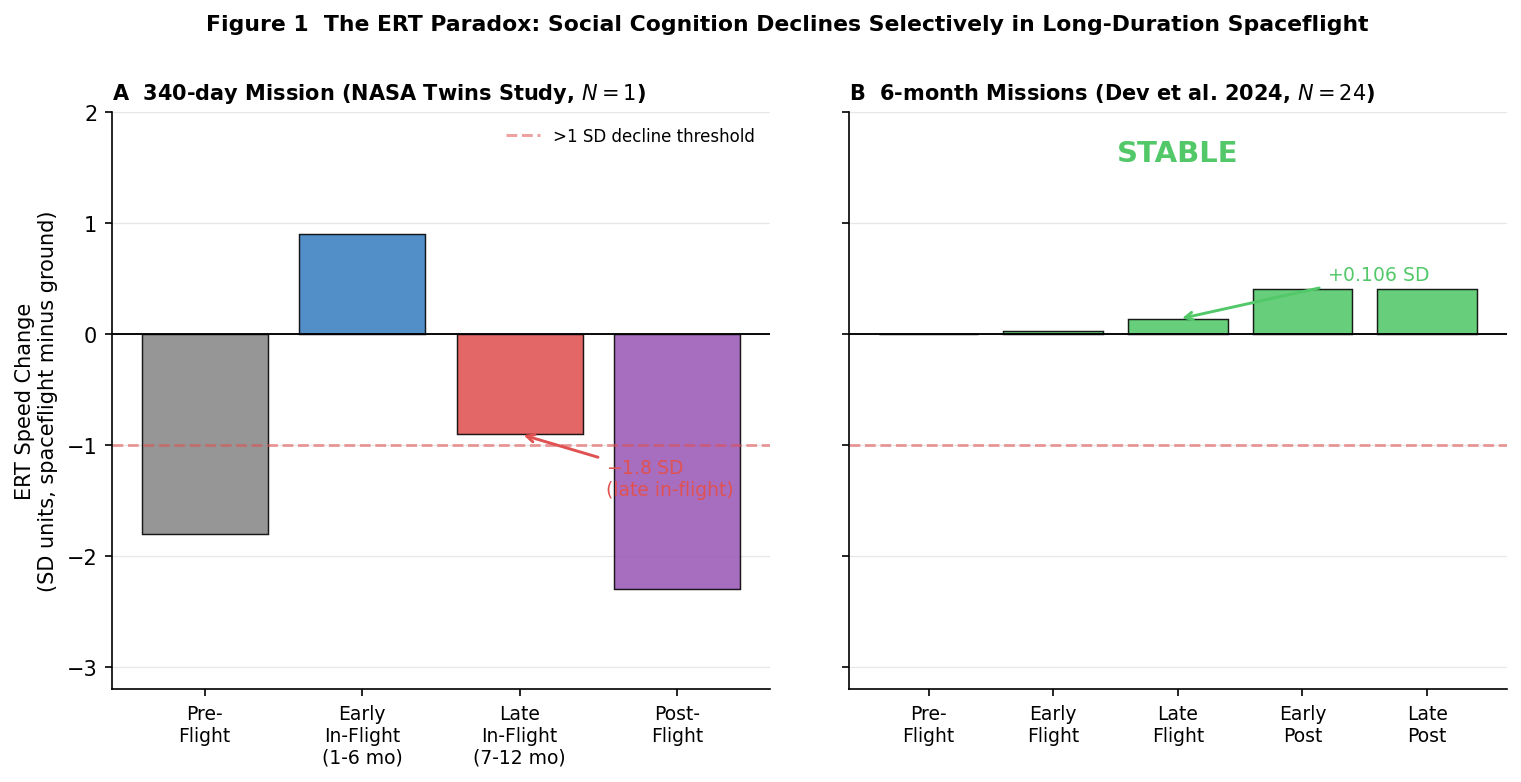
\includegraphics[width=\columnwidth]{fig1_ert_paradox.png}
\caption{\textbf{ERT shows duration-dependent decline.}
\textbf{A:} In 6-month missions ($N=24$), ERT speed is stable throughout
(Dev et al.~2024).
\textbf{B:} In the single-subject 340-day NASA Twins Study, ERT shows the
largest early-to-late inflight decline of any cognitive speed domain
($-1.8$~SD).
Data from Garrett-Bakelman et al.~2019, Figure~10B.}
\label{fig:ert}
\end{figure}

\begin{figure}[H]
\centering
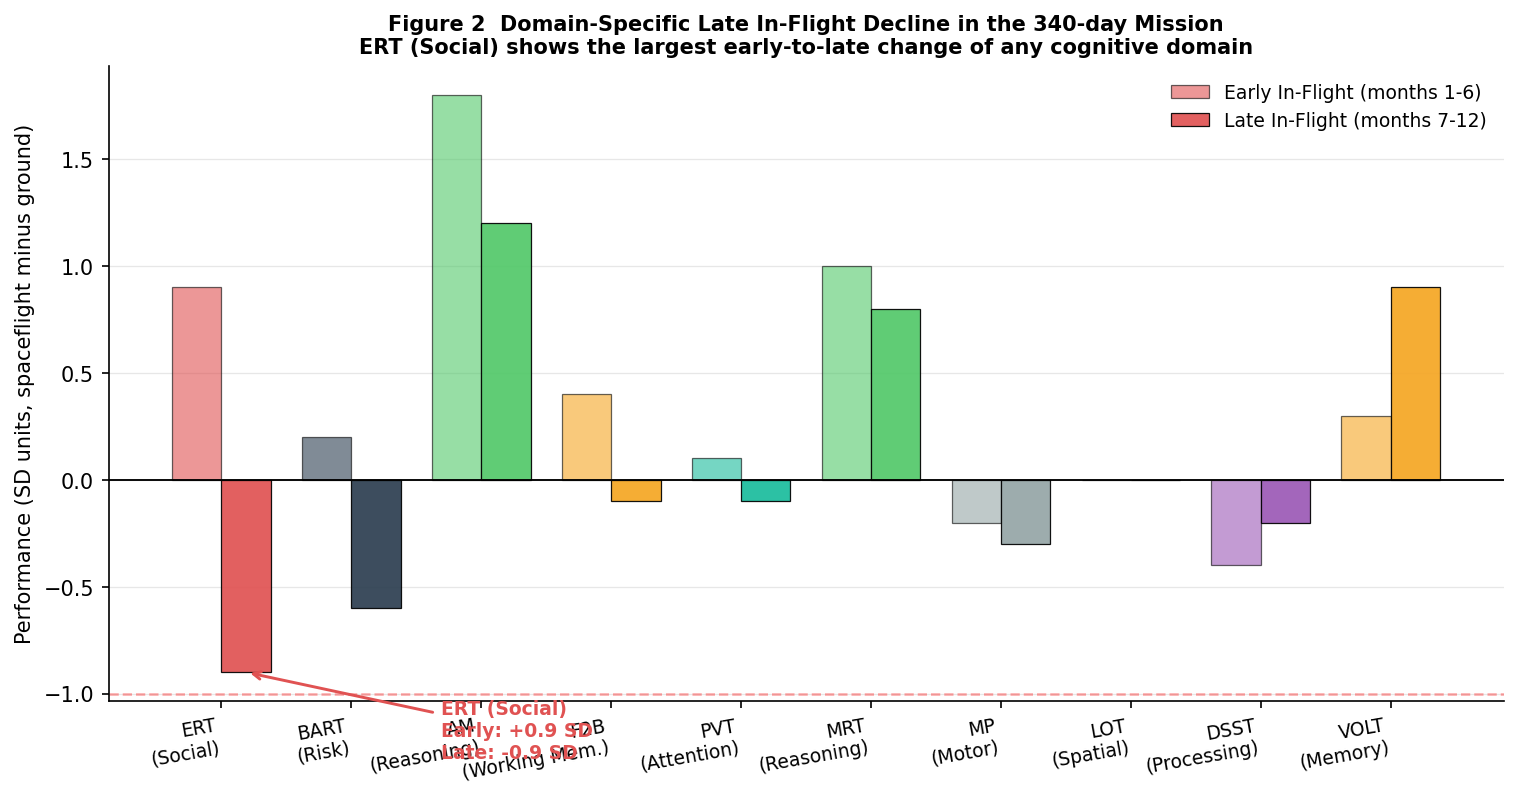
\includegraphics[width=\columnwidth]{fig2_domain_specificity.png}
\caption{\textbf{Domain specificity of ERT decline across all ten cognitive
speed tasks.}
Early-to-late inflight change scores (in SD units) for all 10 NASA
Cognition battery subtests in the single-subject 340-day mission
(Garrett-Bakelman et al.~2019, Figure~10B).
ERT (red) is the most extreme domain by $>$0.7~SD; spatial (LOT: $0.0$~SD)
and visual memory (VOLT: $+0.6$~SD) domains are stable or improving at
the same mission phase.
Dashed line indicates the person-level mean of the nine non-ERT domains.}
\label{fig:domain}
\end{figure}

\subsection{ISS Rodent Tissue Shows a Specific Myelination Signal
Absent in Ground-Based Stress}

In ISS frontal cortex tissue (GSE239336), myelination-associated genes
showed a mean $\log_2$FC of $+0.381$ ($t=3.14$, $p=0.025$; $n=7$ genes),
3.89~SD above the genome-wide null (permutation $p=0.0001$;
Figure~\ref{fig:molecular}).

In the ground-based analogue (OSD-202), the same panel showed a mean
$\log_2$FC of $-0.254$ (one-sample $t$-test: $p=0.008$), but permutation
testing revealed this was not pathway-specific: $-0.88$~SD from the
genome-wide null (permutation $p=0.164$).
The nominal $t$-test significance arose because 54\% of all OSD-202 genes
are slightly downregulated; the myelination panel follows the global trend
rather than showing a specific pathway response.
Notably, the direction of the OSD-202 myelination mean moves with the
genome-wide downtrend rather than opposing it, indicating a qualitatively
distinct molecular response from the ISS upregulation rather than an
attenuated version of it.
This directional reversal is the expected pattern under the VEN Fatigue
Hypothesis, which attributes the ISS myelination upregulation specifically
to gravity-disrupted social cue processing absent in the unloading and
radiation analogue.

Social circuit genes were also specifically upregulated in ISS
tissue ($+0.227$; permutation $p=0.033$; 1.85~SD above null), with no
corresponding signal in ground stress (permutation $p=0.200$).
No other VEN category reached specificity in either rodent dataset.

\begin{figure}[H]
\centering
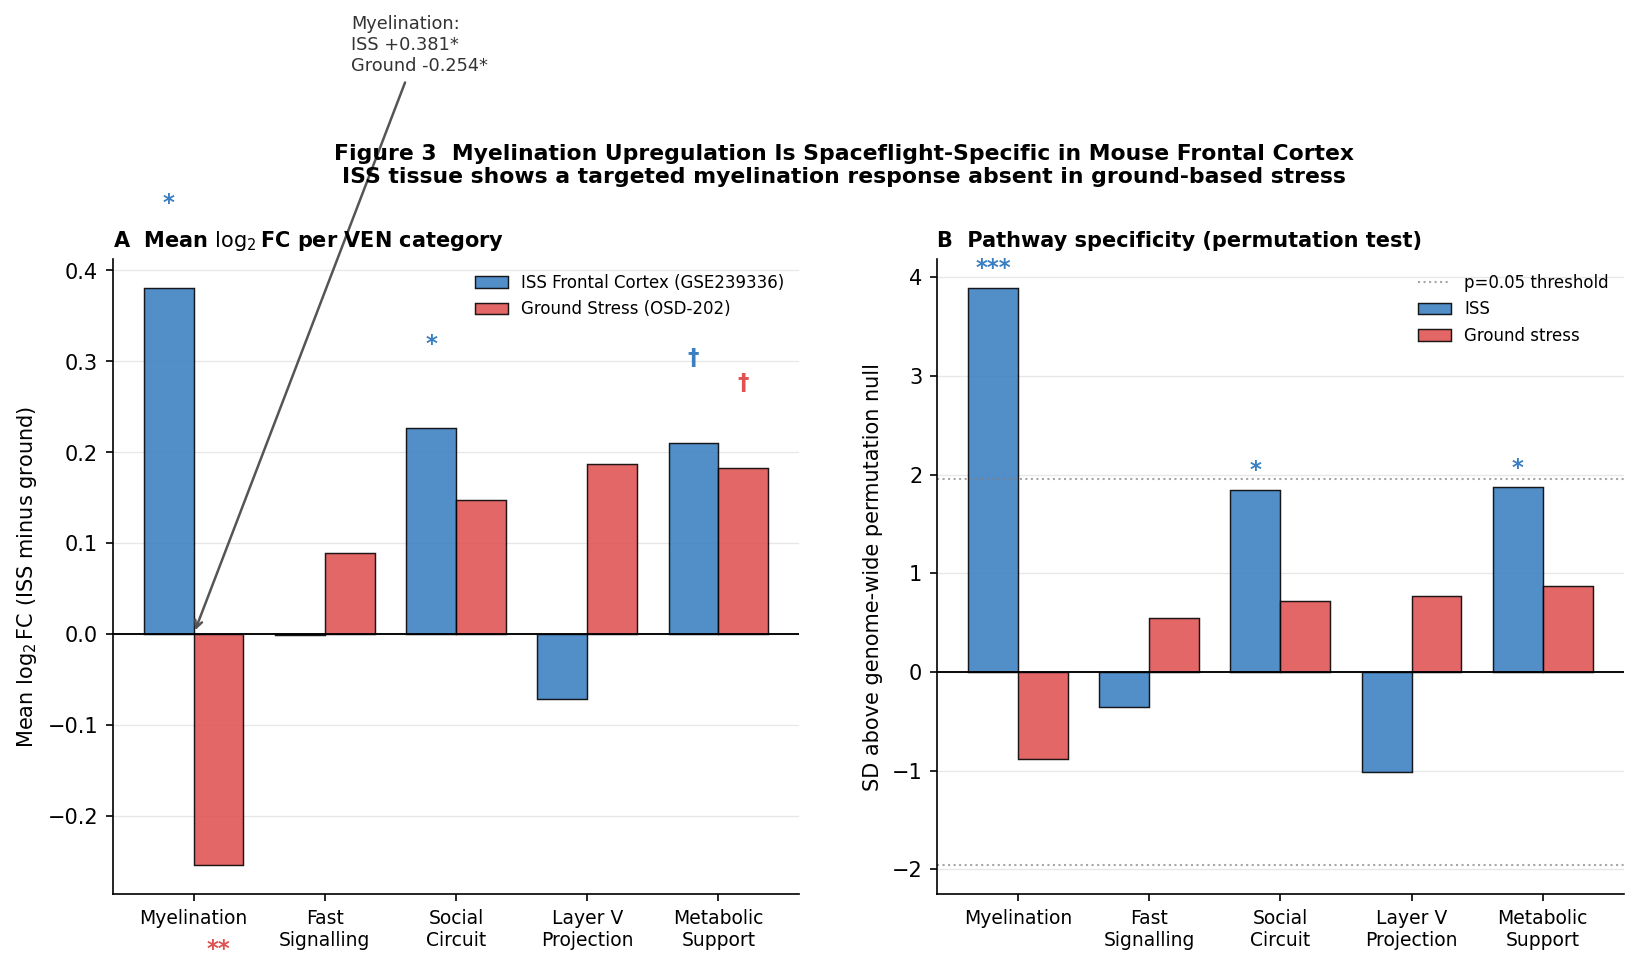
\includegraphics[width=\columnwidth]{fig3_molecular_dissociation.png}
\caption{\textbf{Myelination upregulation is spaceflight-specific in mouse
frontal cortex.}
ISS tissue (GSE239336) shows a specific myelination signal 3.89~SD above
the genome-wide null (permutation $p=0.0001$).
Ground-based spaceflight analogue (OSD-202) shows no specific signal
($-0.88$~SD; permutation $p=0.164$), with the direction of the
myelination mean reversing relative to ISS tissue.
Error bars represent standard error of the permutation null distribution.
Significance markers: $***$ $p<0.001$, $*$ $p<0.05$ (permutation).}
\label{fig:molecular}
\end{figure}

\subsection{Human Cortical Organoids Reveal Specific Layer~V Neuron
Responsiveness to Spaceflight}

All 31~panel genes and NOS1 were detected above the expression threshold
in the GSE259421 count matrix, enabling analysis of all five functional
categories without imputation.
Full results are in Table~\ref{tab:organoid} and Figure~\ref{fig:organoid}.

\textbf{Layer~V Projection genes} showed the strongest signal across all
analyses: combined mean $\log_2$FC $= +1.347$ (6.17~SD above the
genome-wide null; permutation $p=0.0008$, $***$), replicating without
microglia ($+1.423$, $p=0.002$, $**$) and with microglia ($+1.249$,
$p<0.001$, $***$).
The dominant contributors were \textit{BCL11B} ($+4.12$ $\log_2$FC),
\textit{TBR1} ($+2.52$), and \textit{FEZF2} ($+0.46$), master
transcription factors for Layer~V cortical projection neuron
identity~\cite{molyneaux2007}.

\textbf{Metabolic Support genes} were significantly upregulated in the
combined group ($+0.731$; 3.60~SD above null; permutation $p=0.009$,
$**$), driven by \textit{SLC17A7} ($+2.13$), \textit{NRXN1} ($+0.88$),
and \textit{SNAP25} ($+0.51$).

\textbf{Myelination genes} were significantly \emph{downregulated} in
organoids (combined: $-0.456$; $-2.35$~SD below null; permutation
$p=0.035$, $*$), driven by \textit{ERMN} ($-1.60$), \textit{MBP}
($-0.94$), and \textit{PLP1} ($-0.85$).
This direction is opposite to the ISS rodent upregulation and is
interpreted in Section~\ref{sec:disc_org} in light of the \textit{a priori}
prediction stated in Section~\ref{sec:hypothesis}.

\textbf{Social Circuit} genes showed a trend-level upregulation
(combined: $+0.309$; permutation $p=0.098$, $\dagger$).
\textbf{Fast Signalling} genes did not reach specificity
($+0.116$; permutation $p=0.387$).
\textbf{NOS1} showed $+0.541$ $\log_2$FC in the combined group.

\paragraph{Interpretation of permutation and \textit{t}-test results.}
\label{sec:perm_note}
The permutation test and within-panel $t$-test address complementary
questions.
The permutation test assesses whether the VEN category mean exceeds what
is expected from equivalently sized random gene sets drawn from the full
transcriptome (pathway specificity relative to genome-wide background); the
within-panel $t$-test assesses whether individual gene effects are
consistently non-zero across panel members (effect consistency within
the panel).
For Layer~V Projection genes, permutation significance ($p=0.0008$) with a
non-significant within-panel $t$-test ($p=0.189$) reflects that the signal
is concentrated in two genes with very large effects (\textit{BCL11B}:
$+4.12$; \textit{TBR1}: $+2.52$) within a five-gene panel, generating a
high category mean relative to background while limiting power for the
within-panel $t$-test at $n=5$.
Both statistics are reported in Table~\ref{tab:organoid}; permutation
results are emphasised throughout because they directly address the primary
question of pathway specificity rather than within-panel consistency.

\begin{figure}[H]
\centering
\includegraphics[width=\columnwidth]{fig4_organoid_permutation.png}
\caption{\textbf{VEN gene panel permutation specificity in human cortical
organoids (GSE259421).}
Standard deviations above or below the genome-wide null for five VEN gene
categories (combined group, without and with microglia pooled).
Layer~V Projection genes show the strongest signal (6.17~SD above null;
permutation $p=0.0008$).
Myelination genes are significantly below null ($-2.35$~SD; permutation
$p=0.035$), consistent with the \textit{a priori} prediction for immature
organoid models (Section~\ref{sec:hypothesis}).
Significance: $***$ $p<0.001$, $**$ $p<0.01$, $*$ $p<0.05$,
$\dagger$ $p<0.10$ ($N=10{,}000$ permutations, seed 42).}
\label{fig:organoid}
\end{figure}

\subsection{Convergent Patterns Are Consistent with the VEN Fatigue
Hypothesis}

Patterns consistent with both primary predictions were observed across
independent datasets.
H1 received support in rodent frontal cortex: ISS tissue shows a 3.89~SD
specific myelination signal (permutation $p=0.0001$) absent in
ground-based stress (permutation $p=0.164$), with directional reversal in
the analogue consistent with qualitatively distinct rather than merely
attenuated molecular responses.
The human organoid data provide a complementary human cellular finding:
cortical Layer~V projection neurons (the neuronal class from which VENs
are derived) are the most strongly and specifically responsive gene
category to spaceflight conditions (6.17~SD above null; $p=0.0008$);
however, the absence of mature VENs in organoids means this signal
reflects the broader Layer~V projection neuron class and cannot be
attributed specifically to VENs.
H2 received support in the cognitive data: ERT is stable across 6-month
missions ($N=24$) and shows the largest speed change of any domain in the
340-day mission ($t=11.41$, $df=8$; within-individual cross-domain
comparison), consistent with the predicted duration-dependent threshold.

\begin{table*}[t]
\centering
\caption{\textbf{VEN gene panel results in human iPSC-derived cortical
organoids (GSE259421), ISS vs.\ ground control.}
Mean $\log_2$FC = mean of (ISS minus ground) $\log_2$CPM per group.
SD above null = standard deviations of category mean above the
genome-wide permutation null ($N=10{,}000$ random gene sets of equal
size; seed 42).
The permutation test (Perm $p$) assesses pathway specificity relative to
genome-wide background; the within-panel $t$-test ($p$ ($t$-test)) assesses
effect consistency across panel members (see Section~\ref{sec:perm_note}).
Significance: $***$ $p<0.001$, $**$ $p<0.01$, $*$ $p<0.05$,
$\dagger$ $p<0.10$.}
\label{tab:organoid}
\vspace{4pt}
\small
\setlength{\tabcolsep}{5pt}
\begin{tabular}{llrrrrrl}
\toprule
\textbf{Group} & \textbf{Category} & \textbf{$n$} &
\textbf{Mean $\log_2$FC} & \textbf{$t$} & \textbf{$p$ ($t$-test)} &
\textbf{SD above null} & \textbf{Perm $p$}\\
\midrule
Without microglia          & Myelination       & 7 & $-0.462$ & $-1.72$ & 0.141 & $-2.10$ & $0.050^\dagger$ \\
($n_\text{LEO}=4$,         & Fast Signalling   & 7 & $+0.234$ & $+0.64$ & 0.535 & $+1.13$ & 0.192 \\
$n_\text{gnd}=5$)          & Social Circuit    & 6 & $+0.392$ & $+0.59$ & 0.571 & $+1.74$ & $0.077^\dagger$ \\
                           & Layer V Proj.     & 5 & $+1.423$ & $+1.60$ & 0.220 & $+5.72$ & $0.002^{**}$ \\
                           & Metabolic Supp.   & 6 & $+0.947$ & $+2.32$ & 0.064 & $+4.14$ & $0.005^{**}$ \\
\midrule
With microglia             & Myelination       & 7 & $-0.443$ & $-1.79$ & 0.132 & $-2.55$ & $0.028^{*}$ \\
($n_\text{LEO}=5$,         & Fast Signalling   & 7 & $+0.018$ & $+0.05$ & 0.960 & $+0.19$ & 0.784 \\
$n_\text{gnd}=5$)          & Social Circuit    & 6 & $+0.242$ & $+0.50$ & 0.628 & $+1.37$ & 0.137 \\
                           & Layer V Proj.     & 5 & $+1.249$ & $+1.73$ & 0.161 & $+6.27$ & $<0.001^{***}$ \\
                           & Metabolic Supp.   & 6 & $+0.530$ & $+2.43$ & 0.045 & $+2.94$ & $0.017^{*}$ \\
\midrule
Combined                   & Myelination       & 7 & $-0.456$ & $-1.78$ & 0.125 & $-2.35$ & $0.035^{*}$ \\
($n_\text{LEO}=9$,         & Fast Signalling   & 7 & $+0.116$ & $+0.33$ & 0.752 & $+0.66$ & 0.387 \\
$n_\text{gnd}=9$)          & Social Circuit    & 6 & $+0.309$ & $+0.56$ & 0.599 & $+1.56$ & $0.098^\dagger$ \\
                           & Layer V Proj.     & 5 & $+1.347$ & $+1.58$ & 0.189 & $+6.17$ & $0.001^{***}$ \\
                           & Metabolic Supp.   & 6 & $+0.731$ & $+2.44$ & 0.059 & $+3.60$ & $0.009^{**}$ \\
\bottomrule
\end{tabular}
\end{table*}

\begin{table*}[t]
\centering
\caption{\textbf{Key individual VEN marker gene $\log_2$FC in human
cortical organoids (GSE259421), ISS vs.\ ground (combined group).}}
\label{tab:genes}
\vspace{4pt}
\small
\begin{tabular}{llrrr}
\toprule
\textbf{Category} & \textbf{Gene} &
\textbf{$\log_2$FC (no microglia)} &
\textbf{$\log_2$FC (with microglia)} &
\textbf{$\log_2$FC (combined)}\\
\midrule
Myelination       & MBP     & $-0.621$ & $-1.204$ & $-0.941$ \\
                  & PLP1    & $-1.021$ & $-0.702$ & $-0.852$ \\
                  & ERMN    & $-1.765$ & $-1.435$ & $-1.596$ \\
Fast Signalling   & SCN1A   & $+1.196$ & $+0.690$ & $+0.929$ \\
                  & NEFM    & $+1.200$ & $+0.741$ & $+0.955$ \\
Social Circuit    & CHRM1   & $+2.935$ & $+2.069$ & $+2.481$ \\
                  & OXTR    & $-1.741$ & $-1.444$ & $-1.589$ \\
Layer V Proj.     & BCL11B  & $+4.497$ & $+3.729$ & $+4.123$ \\
                  & TBR1    & $+2.929$ & $+2.061$ & $+2.515$ \\
                  & FEZF2   & $+0.448$ & $+0.425$ & $+0.463$ \\
Metabolic Supp.   & SLC17A7 & $+2.825$ & $+1.453$ & $+2.126$ \\
                  & NRXN1   & $+1.102$ & $+0.646$ & $+0.878$ \\
VEN marker (ind.) & NOS1    & $+0.886$ & $+0.234$ & $+0.541$ \\
\bottomrule
\end{tabular}
\end{table*}

\section{Discussion}

\subsection{A Circuit-Level Account of Duration-Dependent Vulnerability}

The ERT paradox (stable performance at six months, selective decline at
twelve months, with other domains unchanged) has not previously received a
mechanistic explanation.
The VEN Fatigue Hypothesis provides a candidate account.
The key insight is that VEN circuits are uniquely sensitive to the quality
of their input because they fire on minimal evidence (fan-in $\approx$8
vs.\ $\sim$80 for pyramidal neurons~\cite{allman2010}).
In normal terrestrial conditions, gravity-calibrated social cues arrive
with high signal fidelity.
In microgravity, these cues are systematically disrupted, requiring the VEN
pathway to fire on noisier inputs and increasing metabolic demand.

Within a six-month mission, the brain may compensate.
The myelination upregulation observed in ISS frontal cortex is consistent
with such compensation: increased myelin deposition accelerates axonal
conduction velocity and reduces energy cost per spike~\cite{purves2018}.
ERT speed is preserved.

Beyond six months, accumulating fatigue may outpace compensation.
A candidate mechanism for this threshold involves the finite capacity of
activity-dependent myelination.
Oligodendrocyte precursors are recruited to myelinate axons in response to
sustained firing, but this precursor pool is not unlimited and mature myelin
synthesis is among the most metabolically expensive biosynthetic processes
in the CNS~\cite{purves2018}.
Under persistent VEN overactivation, the rate of new myelin deposition and
precursor recruitment may eventually lag behind cumulative demand,
particularly as the initial compensatory response exhausts the most
available precursor pool.
A six-month mission may remain within the compensatory envelope; twelve
months may approach or exceed it.
No direct measurements of VEN myelin turnover rates during spaceflight
currently exist, so this threshold account is speculative; however, it
is mechanistically grounded and generates a direct experimental prediction:
measuring oligodendrocyte precursor depletion markers in frontal cortex
tissue from long-duration rodent spaceflight missions would provide a
tractable test.

Other cognitive circuits (including spatial, memory, and reasoning) are not
primarily driven by fast-sparse VEN pathways, and are therefore predicted
to be unaffected at this mission phase.
The result would be ERT-specific late-inflight decline.
Whether this mechanism is the correct explanation requires prospective
studies directly measuring VEN activity and myelin dynamics during
extended spaceflight.

\subsection{Human Organoid Findings: Layer~V Maturation and a Divergent
Myelination Response}
\label{sec:disc_org}

The human cortical organoid data extend this framework to a human cellular
model, with two important contributions and one critical caveat.

The first contribution is the massive, reproducible upregulation of Layer~V
projection genes (\textit{BCL11B}: $+4.12$, \textit{TBR1}: $+2.52$,
\textit{FEZF2}: $+0.46$; combined 6.17~SD above null, $p=0.0008$).
This constitutes preliminary human transcriptomic evidence that the cortical
neuron class from which VENs are derived responds strongly to spaceflight
conditions, consistent with the phenotypic evidence of enhanced cortical
neuron maturation reported by Marotta et al.~\cite{marotta2024}.
Critically, because mature organoids do not contain bona fide VENs (a
specialised cell type requiring specific ACC/frontal insula regional identity
not achieved in standard organoid protocols~\cite{allman2010}), this signal
reflects the broader Layer~V projection neuron class and cannot be attributed
to VENs specifically.

The second contribution is the metabolic support gene upregulation
($+0.731$, $p=0.009$), consistent with increased synaptic activity
in maturing cortical neurons.

The critical caveat concerns the myelination findings.
The direction of the organoid myelination signal ($-0.456$) diverges from
the ISS rodent upregulation ($+0.381$).
Consistent with the \textit{a priori} structural prediction stated in
Section~\ref{sec:hypothesis}, we interpret this contrast mechanistically
rather than as a contradiction.
The VEN Fatigue Hypothesis predicts activity-dependent myelination
upregulation as compensation for sustained elevated VEN firing rates, a
circuit-level demand signal that organoids, being electrically sparse,
immature, and lacking social or vestibular inputs, cannot generate.
The organoid myelination response likely reflects the direct physical
effects of microgravity on oligodendrocyte precursor
differentiation~\cite{marotta2024}, distinct from circuit-level
activity-driven compensation.
This interpretation is supported by the consistency of the myelination
direction across both microglia conditions, ruling out immune-cell
contamination as a primary driver.

\subsection{Why the Myelination Signal Is Spaceflight-Specific}

A critical feature of the rodent molecular results is the contrast between
ISS and ground-stress conditions.
The ISS myelination signal (3.89~SD above the genome-wide null,
$p=0.0001$) is not a general upregulation but a targeted response confined
to the myelination category.
Ground-based stress (hindlimb unloading, radiation) does not produce a
specific signal (permutation $p=0.164$), and the direction of the OSD-202
myelination mean reverses relative to ISS tissue, consistent with a
qualitatively distinct molecular response rather than an attenuated one.

This specificity is mechanistically coherent under the VEN Fatigue
framework.
Ground-based spaceflight analogues stress the body systemically but do not
disrupt gravity-referenced sensory inputs in the same way as orbital
microgravity.
VEN circuits calibrated to gravity-referenced social cues would be
selectively stressed by orbital microgravity but not by mechanical
unloading or radiation, generating a qualitatively distinct molecular
response.

\subsection{Alternative Explanations}
\label{sec:alternatives}

The duration-dependent ERT pattern is consistent with the VEN Fatigue
Hypothesis but is not exclusively explained by it.
Several alternative mechanisms must be considered.

\textbf{General cognitive fatigue.}
Extended confinement, sleep disruption, and psychological stress accumulate
over mission duration and could degrade performance broadly.
However, a domain-general fatigue account predicts multi-domain decline,
whereas spatial and memory domains remain stable or improve during the same
late-inflight phase in which ERT declines; the pattern of domain-selective
vulnerability is difficult to accommodate under a non-specific fatigue
explanation.

\textbf{Cumulative radiation exposure.}
Radiation dose increases with mission duration and has been associated with
biological changes in ISS astronauts~\cite{garrett2019}.
Radiation-induced cognitive effects in animal models, however, are typically
distributed across multiple domains including hippocampally mediated spatial
memory, rather than manifesting as a speed deficit confined to social emotion
recognition alone.

\textbf{Practice and learning effects.}
Repeated administration of the same cognitive battery could produce
performance changes through task familiarity.
Practice effects generally improve performance over time rather than
producing domain-selective late-inflight decline, and the ERT change appears
alongside stability or improvement in other domains assessed with the same
battery at the same time point.

\textbf{Neuroendocrine changes.}
Prolonged spaceflight alters cortisol, thyroid, and other neuroendocrine
profiles~\cite{garrett2019}.
Such changes could plausibly affect neural circuits; however, the
selectivity of the ERT decline for social cognition, measured concurrently
with domains showing no decline, is not straightforwardly predicted by
known neuroendocrine spaceflight effects.

None of these alternatives is ruled out by $N=1$ data.
The VEN Fatigue Hypothesis is advanced as the account that best accommodates
the full pattern of domain-selective, timing-dependent vulnerability; it
is not advanced as an established mechanism.
Controlled prospective studies with larger samples are required to
adjudicate between these accounts.

\subsection{The Duration Threshold}

The data are consistent with a threshold near six months, below which
myelination compensation may be sufficient and above which it may not.
The practical implication is direct: mission planners have long used
six months as a benchmark for Earth orbit stays based on musculoskeletal
and cardiovascular endpoints.
The VEN Fatigue Hypothesis predicts that social cognitive performance
represents an independent limiting factor for missions significantly
beyond this duration, particularly in situations requiring rapid social
judgements such as conflict resolution, group cohesion maintenance, and
emergency decision-making.
A crewed Mars mission at approximately 30~months significantly exceeds
this threshold.

\subsection{Relationship to the Fast Lane Hypothesis SNN Model}

The VEN Fatigue Hypothesis is derived from the Fast Lane
Hypothesis~\cite{keskin2026}, which establishes the circuit-level
prediction that VEN integrity is specifically required for social decision
\emph{speed} but not social cognitive \emph{capacity}.
In the published SNN model~\cite{keskin2026}, the FTD-like versus
Alzheimer's-like double dissociation is central: post-training VEN ablation
(FTD-like) significantly slows social decisions and reduces accuracy
($p<0.0001$), while pyramidal pathway degradation leaving VENs intact
(Alzheimer's-like) does not significantly affect speed ($p=0.68$).
Near-ceiling accuracy across non-FTD conditions confirms that VENs affect
temporal dynamics rather than representational capacity.

These SNN predictions are consistent with the cognitive data: ERT
\emph{speed} declines in late inflight rather than ERT accuracy, consistent
with pathway fatigue rather than the accuracy collapse characteristic of
FTD-like structural VEN loss.
The Alzheimer's-like SNN result provides the inverse prediction: if a
stressor degraded pyramidal pathways while leaving VENs intact, social
decision speed should be preserved, a dissociation that strengthens the
inference that speed-selective ERT decline specifically implicates the VEN
pathway rather than general cortical deterioration.

\subsection{Limitations}

\textbf{$N=1$ for the 340-day cognitive data.}
All 340-day ERT findings derive from a single spaceflight astronaut.
The within-individual cross-domain comparison mitigates but does not
eliminate this fundamental limitation.
These findings must be treated as hypothesis-generating case-study
observations rather than evidence for a general population-level effect;
independent replication in multi-subject long-duration cohorts is the
critical next step.

\textbf{Absence of direct VEN localisation.}
All molecular data derive from bulk tissue or whole-organoid RNA-seq.
We cannot attribute observed changes to VENs specifically, as opposed to
other Layer~V projection neurons or oligodendrocytes.
Future studies using spatial transcriptomics at single-cell resolution or
single-nucleus RNA-seq would be required to localise signals to VEN cell
bodies directly.

\textbf{Cross-species rodent transcriptomics.}
GSE239336 and OSD-202 derive from rodent tissue.
Mouse VEN homologues differ from human VENs in number, regional
distribution, and cytoarchitecture; these findings are presented as
convergent evidence rather than direct mechanistic demonstration in
human tissue.

\textbf{Organoid model limitations.}
The GSE259421 organoids are immature, electrically sparse cellular
aggregates lacking mature cortical lamination, sustained circuit activity,
and bona fide VEN cell types.
Sample sizes are modest ($n=4$--5 per microglia condition), and bulk
RNA-seq cannot resolve cell-type-specific expression changes within the
organoid.

\textbf{Cognitive data digitisation.}
The 340-day cognitive values were manually digitised from Figure~10B
of Garrett-Bakelman et al.~\cite{garrett2019}.
Manual digitisation introduces an estimated uncertainty of approximately
$\pm$0.2~SD in absolute values; at the conservative lower bound of
$-1.6$~SD for ERT, the domain remains the most extreme change by
$>$0.7~SD compared to the next largest (BART: $-0.8$~SD), and all
directional conclusions are preserved.

\textbf{Causal inference.}
All data are observational.
Convergence across four independent lines of evidence is consistent with
the VEN Fatigue Hypothesis but does not establish it.
Prospective studies directly measuring VEN pathway function and myelin
dynamics during extended spaceflight are required to test causal claims.

\section{Conclusion}

A previously unresolved paradox in spaceflight cognition research (why
social cognition is specifically stable within 6-month missions but
specifically vulnerable beyond that threshold) motivates the VEN Fatigue
Hypothesis: duration-dependent selective vulnerability may arise because
VEN circuits, optimised for fast social decisions on minimal evidence, are
overactivated by gravity-disrupted social cues beyond a 6-month threshold
at which myelination compensation becomes insufficient.

This hypothesis is motivated by four convergent but indirect lines of
evidence.
First, in the single-subject 340-day NASA Twins Study, ERT speed shows
the largest early-to-late inflight decline of any cognitive speed domain
($-1.8$~SD; within-individual cross-domain comparison: $t=11.41$, $df=8$)
while remaining stable across 6-month missions ($+0.106$~SD; $N=24$).
Second, ISS frontal cortex tissue shows a specific myelination upregulation
3.89~SD above the genome-wide null (permutation $p=0.0001$) that is absent
in a ground-based spaceflight analogue (permutation $p=0.164$), with
directional reversal in the analogue consistent with a qualitatively
distinct molecular response.
Third, human iPSC-derived cortical organoids on the ISS show massive
upregulation of Layer~V projection genes ($+1.347$ $\log_2$FC; 6.17~SD
above null; permutation $p=0.0008$), providing preliminary human
transcriptomic evidence of spaceflight responsiveness in the neuronal class
from which VENs are derived; the accompanying myelination downregulation
is consistent with an \textit{a priori} prediction for circuit-inactive
organoid models.
Fourth, the Fast Lane Hypothesis SNN model~\cite{keskin2026} provides
the theoretical circuit-level framework connecting VEN integrity to social
decision speed rather than capacity.

Together, these findings motivate a circuit-grounded framework for
duration-dependent cognitive risk in human spaceflight and point toward
testable countermeasure strategies and prospective study designs for
missions beyond the six-month threshold.

\bibliographystyle{unsrtnat}
\bibliography{references}

\end{document}
